In this chapter we come to the core of this thesis, namely the empirical performance investigation of the Fribourg construction. The aim of this investigation is to find out how the Fribourg construction performs on \textit{actual} automata. This is opposed to the theoretical investigation of the worst-case performance, which reveals how the construction performs on a specific \textit{worst-case} automaton. The goal of this chapter is to describe in detail the empirical study that we carried out. The actual results of the investigations are presented in Chapter~\ref{chap_results}.

For investigating the performance of the Fribourg construction, we proceed in two tracks. First, we want to test the Fribourg construction with its different combinations of optimisations and compare them to each other. Second, we want to compare the Fribourg construction with other complementation constructions. We refer to the first track of investigation as the \textit{internal tests}, and to the second track as the \textit{external tests}. Note that our main performance measure is the number of states of the complement automaton. However, we sometimes also use the execution times of complementation taks as a secondary measure.

For an empirical performance investigation of a Büchi complementation construction, one needs basically three things: an implementation of the construction, test data, and an experimental setup, including an execution environment. Regarding the \textit{implementation}, we decided to create it as a part of the \goal{} tool. \goal{} is an \om-automata tool, which has already been used previously for empirical investigations of Büchi complementation constructions (see Section~\ref{1_empirical}). Furthermore \goal{} contains many pre-implemented complementation constructions, so that, for the external tests, we can run all the tested complementation constructions in a common framework.

\textit{Test data} means basically a set of concrete automata that are given as input to a construction, in order to analyse the output of the construction. We use two different test sets for our investigation, that we refer to as the \goal{} test set and the Michel test set (consisting of Michel automata~\cite{michel1988}). The automata of both test sets have been used in previous investigations of Büchi complementation construction by other authors (see Section~\ref{1_empirical}). We believe that the use of test data that has been previously used increases the validity of our results, as they can be compared to related work.

Our \textit{experimental setup} includes a definition of the concrete tests that are run, that is, which construction, or version of a construction, is executed on which test data. It also states time and memory limits that are impopsed on the experiments, and specifies the execution environment. Regarding the execution environment, since our study includes in large computations, we decided to use professional high-performance computing (HPC) facilities. Concretely, we execute all the experiments on a Linux-based HPC cluster named UBELIX of the University of Bern\footnote{\url{http://ubelix.unibe.ch}}.

% Having an implementation and test data, the experiments need to be executed. Our chosen implementation approach and test data results in heavy computation tasks, that require a lot of computation power and time. We therefore decided to execute the experiments in a professional high-performance computing (HPC) environment. This environment is the Linux-based HPC computing cluster, called UBELIX, at the University of Bern.\footnote{\url{http://ubelix.unibe.ch}}

In this chapter, we discuss each of the mentioned points in more detail. We treat the implementation of the Fribourg construction in Section~\ref{4_impl}, the test data in Section~\ref{4_test_data}, and the experimental setup in Section~\ref{4_exp_setup}.


\section{Implementation}
\label{4_impl}
As mentioned, we implemented the Fribourg construction as part of the \goal{} tool. In this section, we first present the \goal{} tool in a general way (Section~\ref{4_goal}). In Section~\ref{4_implementation}, we describe how we implemented the Fribourg construction with its optimisations as a part of this tool. Clearly, an implementation is only useful if it is correct. Therefore, in Section~\ref{4_verification}, we describe how we verified the correctness of our implementation.


\subsection{The GOAL Tool}
\label{4_goal}
\goal{} stands for \textit{Graphical Tool for Omega-Automata and Logics} and is being developed at the Department of Information Management at the National Taiwan University (NTU)\footnote{\url{http://exp.management.ntu.edu.tw/en/IM}}. The tool has been described in various scientific publications~\cite{2007_goal,2008_goal_ext,2009_goal,2013_goal}. The \goal{} tool is freely available on \url{http://goal.im.ntu.edu.tw}. It is a Java program, and thus runs on every platform having a Java Runtime Environment (JRE).

\goal{} is a graphical and interactive tool for creating and manipulating \om-automata. It provides a large number of operations that can be applied to these automata. These operations range from input testing, conversions to other types of \om-automata, to union and intersection. Figure~\ref{goal_gui} shows a screenshot of \goal's graphical user interface with an open menu showing the breadth of operations that \goal{} provides. Of course, complementation is also part of these operations, and \goal{} includes implementations of many existing Büchi complementation constructions. We will discuss the complementation constructions that \goal{} provides further below.

\begin{figure}[htb!]
\centering
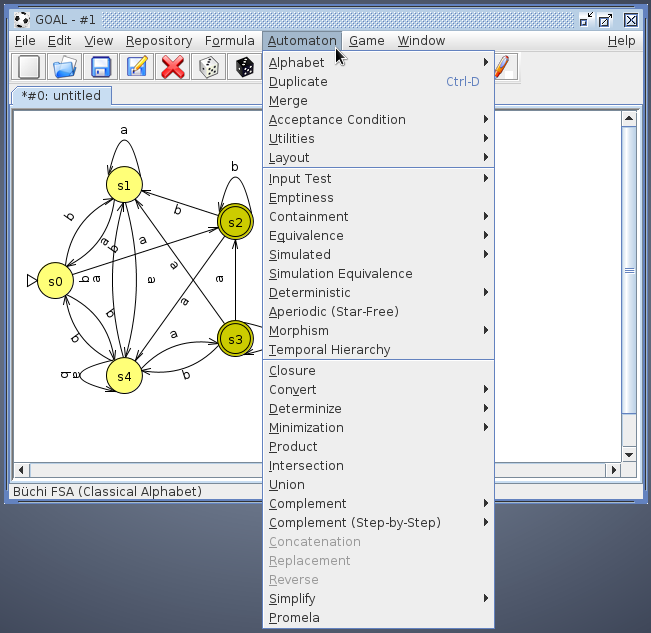
\includegraphics[width=0.45\textwidth]{figures/goal.png}
\caption{The graphical user interface of \goal{} (version 2014--11--17). The open menu item gives an idea about the different types of manipulations that can be applied to \om-automata.}
\label{goal_gui}
\end{figure}

The versions of \goal{} have names of the form YYYY--MM--DD that correspond to the release date of the version. The latest version at the time of this writing, and the version that we used in our experiments, is 2014--11--17.

Automata can be imported to and exported from \goal{} in different formats. The default format is the \goal{} File Format (GFF). Files of the GFF type have by convention the extension ``.gff''. 

As mentioned, \goal{} has a graphical user interface, as shown in Figure~\ref{goal_gui}. However, almost the entire functionality of \goal{} is also available through a command line interface. For example, complementing an automaton can then be done with the command \textsf{gc complement -m safra -o out.gff in.gff} from the commandline. The effect of this command is to complement the automaton in the file \textsf{in.gff} with Safra's complementation construction, and write the complement automaton to the file \textsf{out.gff}. The command \textsf{gc} is the entry point to \goal's command line interface. For our empirical performance investigation, we use the command line interface of \goal.

Let us now have a closer look at the Büchi complementation constructions that are pre-implemented in \goal. The 2014--11--17 version of \goal{} provides a number of 10 complementation constructions. We list these constructions along with their authors and reference to the literature in Table~\ref{goal_constructions}.

\begin{table}[htb!]
\centering
\begin{tabular}{lllr}
\hline
Identifier & Description & Authors (year) & Reference \\
\hline
Ramsey        & Ramsey-based construction & Sistla et al. (1987)
              & \cite{1985_sistla,PrasadSistla1987217} \\
Safra         & Safra's construction & Safra (1988)
              & \cite{1988_safra_2,1988_safra_1} \\
ModifiedSafra & Slightly modified Safra's construction & Althoff et al. (2006)
              & \cite{2006_althoff} \\
Piterman      & Safra-Piterman construction & Piterman (2007)
              & \cite{2006_piterman,2007_piterman} \\
MS            & Muller-Schupp construction & Muller, Schupp (1995)
              & \cite{Muller199569} \\
Rank          & Rank-based construction & Schewe (2009)
              & \cite{schewe2009buchi} \\
WAA           & Via weak alternating automata & Kupferman, Vardi (1997/2001)
              & \cite{1997_vardi,Kupferman:2001} \\
WAPA          & Via weak alternating parity automata & Thomas (1999)
              & \cite{1999_thomas} \\
Slice+P       & Slice-based construction & Vardi, Wilke (2007)
              & \cite{vardi2007automata} \\
Slice         & Enhanced slice-based construction & Kähler, Wilke (2008)
              & \cite{2008_kaehler} \\
\hline
\end{tabular}
\caption{The Büchi complementation constructions provided by \goal{} version 2014--11--17.}
\label{goal_constructions}
\end{table}

As can be seen in Table~\ref{goal_construction}, almost all complementation constructions that \goal{} provides have been reviewed in Section~\ref{2_review}. The only exception is ModifiedSafra, which is a minor modification to Safra's construction that has been proposed by Althoff et al.~\cite{2006_althoff}. Furthermore, \goal{} has at least one construction of each of the four main complementation approaches. Ramsey belongs to the Ramsey-based approach, Safra, ModifiedSafra, Piterman, and MS belong to the determnisation-based approach, Rank, WAA, and WAPA to the rank-based approach, and Slice and Slice+P to the slice-based approach. Note that the identifiers that are defined in Table~\ref{goal_constructions} for each construction are also used by \goal, and we will use them throughout this thesis to refer to the corresponding constructions.

The construction Slice+P is actually the construction Slice with the P option. That is, from the perspective of \goal, there is only the single construction Slice, however, if the P option is specified, then the slice-based construction by Vardi and Wilke~\cite{vardi2007automata} is used, and otherwise the slice-based construction by Kähler and Wilke \cite{2008_kaehler} is used.

% We sorted the construction in Table~\ref{goal_constructions} according to the four fundamental complementation approaches, Ramsey-based, determinization-based, rank-based, and slice-based. The first construction, Ramsey, is the only construction belonging to the Ramsey-based complementation approach. The following four constructions, Safra, ModifiedSafra, Piterman, and MS, belong to the determinization-based approach. Rank, WAPA, and WAA belong to the rank-based approach. Finally, Slice and Slice+P belong to the slice-based approach. Throughout the rest of this thesis, when we refer to one of \goal's Büchi complementation constructions, we will use the identifiers as defined in Table~\ref{goal_constructions}.

% Safra's construction is in fact a determinization construction that converts a non-deterministic Büchi automaton to a deterministic Rabin automaton. The deterministic Rabin automaton can be trivially complemented to a deterministic Streett automaton by replacing the Rabin acceptance condition with a Streett acceptance condition. Finally, the deterministic Streett automaton is converted to a non-deterministic Büchi automaton.

% ModifiedSafra uses the same procedure as Safra with the difference that a modified version of Safra's construction for converting a NBW to a DRW is used.

% Slice and Slice+P are actually combined in a single construction in \goal. However, one of the two constructions can be selected by the means of the option P. With the P option, the construction by Vardi and Wilke is used, and without the P option, the one by Kähler and Wilke is used. For our study, we will use Vardi and Wilke's construction (with the P option), however, we will usually still refer to this construction as simply Slice.

At this point, it is worth pointing at a related project of the same research group, called the \textit{Büchi Store}~\cite{2011_buchi_store}. This is an online repository of categorised \om-automata that can be downloaded in different formats (including GFF). The Büchi Store is accessible over the web on \url{http://buchi.im.ntu.edu.tw/}. Furthermore, there is a binding in \goal{} to the Büchi Store, so that automata can be directly downloaed into \goal. For our study we did not use the Büchi Store, but it is might be an interesting option for future work.


\subsection{Implementation of the Construction}
\label{4_implementation}
\subsubsection{The \goal{} Plugin Architecture}
\goal{} has been designed from the ground up to be modular and extensible. To this end, it has been created with the Java Plugin Framework (JPF)\footnote{\url{http://jpf.sourceforge.net/}}. This framework allows to build applications whose functionality can be easily and seamlessly extended by writing plugins for it. These plugins can be installed in the main application without the need to recompile the whole application. Rather, the plugin is compiled separately and the resulting bytecode files are copied to the directory tree of the main application. It is not even necessary to know the source code of the main application in order to write a plugin. The interfaces of JPF itself, and the documentations of the relevant classes of the main application are all that plugin writers need to know.

In some more detail, JPF requires an application to define so called \textit{extension points}. For any extension point, multiple \textit{extensions} can be provided. These extensions contain the actual functionality of the application. A JPF application basically consists of extensions that are plugged into their corresponding extension points. A plugin is an arbitrary bundle of extensions and extension points. It is the basic unit of organisation in the Java Plugin Framework.

One of the extension points of \goal{} is called \textsf{ComplementConstruction}. The extensions to \textsf{ComplementConstruction} contain the actual complementation constructions that \goal{} provides. For adding a new complementation construction to \goal, one has thus to create a new extension to \textsf{ComplementConstruction}. This extension can then be wrapped in a plugin, and the plugin can be compiled and installed in the main application, what makes it an integral part of it. This means that once the plugin is installed, the new construction is included in \goal{} in the same way as all the other constructions.

It is thanks to this open architecture of \goal{} that welcomes extension that we were able to seamlessly add the Fribourg construction to this tool. In particular, we created a \goal-plugin that contains the implementation of the Fribourg construction. We present this plugin below.

\subsubsection{The Fribourg Construction Plugin}
The name of our plugin containing our implementation of the Fribourg construction is \textsf{ch.unifr.goal.complement}\footnote{By convention, JPF plugins are named after the corresponding Java package.}. The plugin is freely available and can be installed by any \goal{} user. The installation in \goal{} is very easy. We give instructions on how to obtain, install, and use the plugin in Appendix~\ref{app_plugin}.

We aimed at fully integrating the Fribourg construction in \goal. The current version of the plugin includes menu integration of the Fribourg construction, the pertinent saving of option defaults, and a step-by-step execution facility for the Fribourg construction. This last point is a great way for learning how the Fribourg construction works.

Our implementation of the Fribourg construction also includes the three optimisations R2C, M1, and M2 that we described in Section~\ref{3_optimisations}. These optimisations are freely selectable by the user and can be combined in different ways. In the GUI, the optimisations are presented to the user as selectable check boxes before the start of the construction. In the command line mode, they can be set as flags of the entered command.

In addition to these three optimisations, we added further options to our construction. Table~\ref{goal_options} provides a listing of all of them. Note that each option has an identifier consisting of upper-case letters. We use these identifiers throughout the rest of this thesis to refer to the corresponding options.

\begin{table}
\centering
\begin{tabular}{ll}
\hline
Option & Description \\
\hline
R2C  & Apply R2C optimisation \\
M1   & Apply M1 optimisation \\
M2   & Apply M2 optimisation  \\
C    & Make input automaton complete \\
R    & Remove unreachable and dead states from output automaton \\
RR   & Remove unreachable and dead states from input automaton \\
MACC & Maximise accepting states of input automaton \\
B    & Use the ``bracket notation'' for state labels \\
\hline
\end{tabular}
\caption{The options for the Fribourg construction in our Fribourg construction plugin for \goal.}
\label{goal_options}
\end{table}

We discuss each of the options in Table~\ref{goal_options} below. The first three options are the three optimisations to the Fribourg construction that we described in Section~\ref{3_optimisations}. The R2C optimisation is implemented so that it applies only to input automata that are complete. That is, if R2C is activated for the complementation of an automaton that is not complete, then this option has no effect. The options M1 and M2 stand for the M1 and M2 optimisations. Since M2 is dependent on M1, it is not possible to select M2 without also selecting M1. This restriction is enforced in both the GUI and the command line interface.

The C option is one of the options that modifies the input automaton before the actual complementation starts. This option first checks if the input automaton is complete, and if this is not the case, makes it complete by adding a sink state. The purpose of the C option is to be used in conjunction with the R2C optimisation. Making an automaton complete before the start of the construction ensures that the R2C optimisation will be applied. The question arises whether, in terms of performance, it is worth to do this, because making an automaton complete increases its size by one, what increases the potential size of the output automaton. This question has been investigated in previous work on the Fribourg construction by Göttel~\cite{2013_bsc_goettel}. In this thesis will re-investigate this point in an extended form (see Section~\ref{4_exp_setup}).

The R option modifies the output automaton at the end of the construction. In particular, it removes all the so called unreachable and dead states from the complement. Unreachable states are states that cannot be reached from the initial state. Dead states are states from which it is not possible to reach an accepting state. These states can be removed from any automaton without changing the language of the automaton. The pre-implemented complementation constructions Ramsey, Piterman, Rank, and Slice contain a similar R option.

An exmple usage case of the R option is to investigate the number of unreachable and dead state that a complementation construction produces. A way to do this is to complement the same automaton with and without the R option, and calculating the difference of the sizes of the two complements. Such investigations have been done with by Tsai~et~al.~\cite{2011_tsai} in their comparative study of several Büchi complementation constructions in \goal. We will do similar investigations, although it is not the main focus of our study.

The RR option is similar to the R option, with the difference that it removes the unreachable and dead states from the input automaton rather than from the output automaton. This option is not common among the other complementation constructions in \goal, and we are not using it in our study.

The MACC option is again an option that modifies the input automaton before the start of the construction. It maximises the accepting set of the input automaton. This means that as many states as possible are made accepting so that the language of the automaton is not changed. The idea is that the larger number of accepting state simplifies the complementation task. This technique has been introduced and empirically investigated by Tsai~et~al.~\cite{2011_tsai}. The pre-implemented complementation constructions Ramsey, Piterman, Rank, and Slice also contain the MACC option. In our study we will however not use the MACC option.

Finally, the B option only affects the formatting of the labels of the output-states. It has no effect on the consruction itself. In particular, it activates the bracket notation, which is an informal alternative way to indicate the colours of components of states. It does so by using different types of brackets for the subsets, rather than wrapping the subset in a tuple with the colour number, like the default notation.


\subsection{Verification of the Implementation}
\label{4_verification}
% Results on  UBELIX/jobs/2014-11-25
It is important to verify that our implementation of the Fribourg construction is correct. The construction is correct if the output automata it produces are really the complements of the corresponding input automata. Note that this is not the same sense of correctness as the verification that our implementation faithfully represents the specification of the construction. However, with regard to the fact that our implementation produces correct complements, we believe that this is also the case.

In order to verify that our implementation produces correct complements, we performed so called complementation-equivalence tests in \goal. This works as follows. Take an automaton $A$ and complement it with one of the existing constructions in \goal, resulting in the complement automaton $B^\prime$. Then, complement the same automaton $A$ with our implementation of the Fribourg construction, which yields the automaton $B^{\prime\prime}$. Now, by the means of \goal's equivalence operation test whether $A^\prime$ and $A^{\prime\prime}$ are equivalent. If yes, then our implementation produced a correct complement.

This approach makes a couple of assumptions. First, it relies on the correctness of the pre-implemented complementation constructions, and on the equivalence operation of \goal{} (which is also based on complementation). Second, with this empirical approach it is not possible to conclusively verify the correctness of our implementation. Every passed complementation-equivalence test just further confirms the hypothesis that our implementation is correct, but it can never be proved. Despite these issues, a sufficient number of passed tests, still makes us sufficiently confident that our implementation is correct.

We tested the Fribourg construction in different versions with all the options that we described in the last section (except the B option as it does not influence the construction). The tested versions are the following.
\begin{itemize}
\item Fribourg
\item Fribourg+R2C+C
\item Fribourg+M1
\item Fribourg+M1+M2
\item Fribourg+R
\item Fribourg+RR
\item Fribourg+MACC
\end{itemize}

We tested each version with 1,000 randomly generated automata. The automata had a size of 4 and an alphabet size between 2 and 4. The pre-implemented that we used as the ground-truth is Piterman. The result was that all the tests were successful. 

With four states, the automata used for the tests are rather small, and it would be interesting to do the tests with larger automata. However, our limited computing and time resources prevented us from doing so. The equivalence test of \goal{} is implemented as reciprocal containment tests, which in turn is based on complementation. This means that the equivalence test includes the complementation of the complements of the test automata. By using larger test automata, their complements might be already so large that a further complementation is practically infeasible with our available resources. Nevertheless, we think that the number of passed tests with these small automata indicates the absence of implementation errors with a high probability.


\section{Test Data}
\label{4_test_data}
After an implementation, the test data is the second main ingredient of an empirical performance investigation. The test data consists of the sample automata that are given as input to the construction, in order to analyse the produced output. The test data is an important part of every empirical study and should meet several requirements: it should include enough test cases so that the results are significant, it should not be biased in favour of the tested algorithm, and it should cover test scenarios that are relevant for evaluating the performance of the tested algorithm. The ideal case is to use publicly available test data, that has been previously used for other studies. In this way, the test data can be critically inspected by everybody, and furthermore the results of the study are comparable to the results of other studies.

We decided to use two sets of test data that have both been used in other studies. The first is the \goal{} test set, that has been created by Tsai et al.~\cite{2011_tsai}, and used in other studies, such as~\cite{2012_breuers} and~\cite{2013_bsc_goettel}. It consists of 11,000 non-deterministic Büchi automata of size 15. The second set of automata, which we call Michel test set, consists of the smallest four Michel automata. Michel automata are the automata that Michel used to prove the lower bound of $n!$ for the worst-case state complexity of Büchi complementation~\cite{michel1988}. The Michel automata have been used as the test data for other empirical studies, such as~\cite{2006_althoff}, or~\cite{2013_bsc_goettel}. In the following subsections, we first describe the \goal{} test set, and then our used Michel test set.

Test sets available: 

GOAL: \url{https://frico.s3.amazonaws.com/test_sets/goal.zip}

Michel: \url{https://frico.s3.amazonaws.com/test_sets/michel.zip}


\subsection{GOAL Test Set}
\label{4_goal_testset}
The \goal{} test set is the larger and more complex one of the two test sets. In this section, we first introduce the \goal{} test set and describe its basic structure. In the second part, we present the results of an analysis that we did in order to reveal further properties of the \goal{} test set, namely the number and distribution of complete, universal, and empty automata.

\subsubsection{Structure}
The \goal{} test set has been created by Tsai~et~al.~\cite{2011_tsai} for an empirical study evaluation the effects of several optimisations on existing Büchi complementation constructions. This study has been executed in \goal{} and the automata in the test set are available in the \goal{} file format. This is why we call the data \goal{} test set.

The \goal{} test set consists of 11,000 automata of size 15\footnote{There exists a second version with 11,000 automata of size 20.}. It is available through the following link: \url{https://fribourg.s3.amazonaws.com/testset/goal.zip}\footnote{This link is maintained by the author of the thesis. The link to the original location of the  \goal{} test set is \url{http://goal.im.ntu.edu.tw/wiki/lib/exe/fetch.php?media=goal:ciaa2010_automata.tar.gz}. This package contains additionally the second version of the \goal{} test set with the 11,000 automata of size 20.}. All the automata in the test set have 15 states and an alphabet size of 2 (consising of the symbols 0 and 1). The further properties of the automata, namely accepting states and transitions, are determined by the values of two parameters called \textit{transition density} and \textit{acceptance density}

The transition density determines the number of transitions of an automaton. In particular, the transition density $t$ is defined as follows. Let $n$ be the number of states of automaton $A$, and $t$ its transition density. Then $A$ contains $tn$ transitions for each symbol of the alphabet. In the case that $tn$ is not an integer, it is rounded up to the next integer. That is, if one of our automata with 15 states and the alphabet ${0, 1}$ has a transition density of 2, then it contains exactly 30 transitions for symbol $0$ and 30 transitions for symbol $1$. %At creation time the start and end points of these transitions are chosen at random. %Consequently, each state has on average two outgoing and two incoming transitions for each symbol. Therefore, the transition density can also be seen as the average number of outgoing and incoming transitions per alphabet symbol that a state has.

The acceptance density $a$ is defined as the ratio of accepting states to non-accepting states in the automaton. It is thus a number between 0 and 1. If automaton $A$ has $n$ states and an acceptance density of $a$, then it has $an$ accepting states. In the case that $an$ is not an integer, it is rounded up to the next integer. For example, an automaton of the test set with an acceptance density of 0.5 contains 8 accepting states. %Which $an$ states are made accepting is determined randomly at creation time.

The \goal{} test set is structured into 110 classes with different transition density/acceptance density pairs. These 110 pairs result from the Cartesian product of 11 transition densities and 10 acceptance densities. The concrete transition densities $t^\prime$ and acceptance densities $a^\prime$ are the following:
\begin{align*}
t^\prime & = \left( 1.0,\,1.2,\,1.4,\,1.6,\,1.8,\,2.0,\,2.2,\,2.4,\,2.6,\,2.8,\,3.0 \right) \\
a^\prime & = \left( 0.1,\,0.2,\,0.3,\,0.4,\,0.5,\,0.6,\,0.7,\,0.8,\,0.9,\,1.0 \right)
\end{align*}
Thus, there is one class whose automata have a transition density of 1.0 and an acceptance density of 0.1, another class with a transition density of 1.0 and an acceptance density of 0.2, and so on. Each of the 110 classes contains 100 automata. According to~\cite{2011_tsai}, these parameter values were chosen to provide a broad range of complementation problems ranging from easy to hard.


\subsubsection{Completeness, Universality, and Emptiness}

\renewcommand{\tabcolsep}{0.05cm}   % Change table spacings
\renewcommand{\arraystretch}{1.05}
\newcolumntype{R}{>{\raggedleft\arraybackslash}p{1.5em}}
\begin{figure}[htb!]
  \centering
  \begin{subfigure}{\textwidth}
    \begin{subtable}{0.47\textwidth}
    % latex table generated in R 3.1.2 by xtable 1.7-4 package
% Sun Aug 16 12:48:04 2015
\begin{tabular}{r|RRRRRRRRRR}
  & 0.1 & 0.2 & 0.3 & 0.4 & 0.5 & 0.6 & 0.7 & 0.8 & 0.9 & 1.0 \\ 
  \hline
1.0 & 0 & 0 & 0 & 0 & 0 & 0 & 0 & 0 & 0 & 0 \\ 
  1.2 & 0 & 0 & 0 & 0 & 0 & 0 & 0 & 0 & 0 & 0 \\ 
  1.4 & 0 & 0 & 0 & 0 & 0 & 0 & 0 & 0 & 0 & 0 \\ 
  1.6 & 0 & 0 & 0 & 0 & 0 & 0 & 0 & 0 & 0 & 0 \\ 
  1.8 & 1 & 1 & 0 & 0 & 0 & 1 & 1 & 1 & 0 & 0 \\ 
  2.0 & 0 & 5 & 1 & 2 & 2 & 3 & 1 & 2 & 2 & 2 \\ 
  2.2 & 5 & 10 & 8 & 5 & 3 & 5 & 8 & 6 & 7 & 1 \\ 
  2.4 & 10 & 6 & 11 & 11 & 8 & 6 & 10 & 20 & 9 & 7 \\ 
  2.6 & 17 & 17 & 12 & 16 & 14 & 19 & 22 & 21 & 19 & 19 \\ 
  2.8 & 27 & 20 & 29 & 32 & 26 & 27 & 30 & 25 & 24 & 19 \\ 
  3.0 & 37 & 37 & 40 & 39 & 34 & 37 & 38 & 35 & 38 & 39 \\ 
  \end{tabular}

    \end{subtable}
    \hfill
    \begin{subfigure}{0.52\textwidth}
    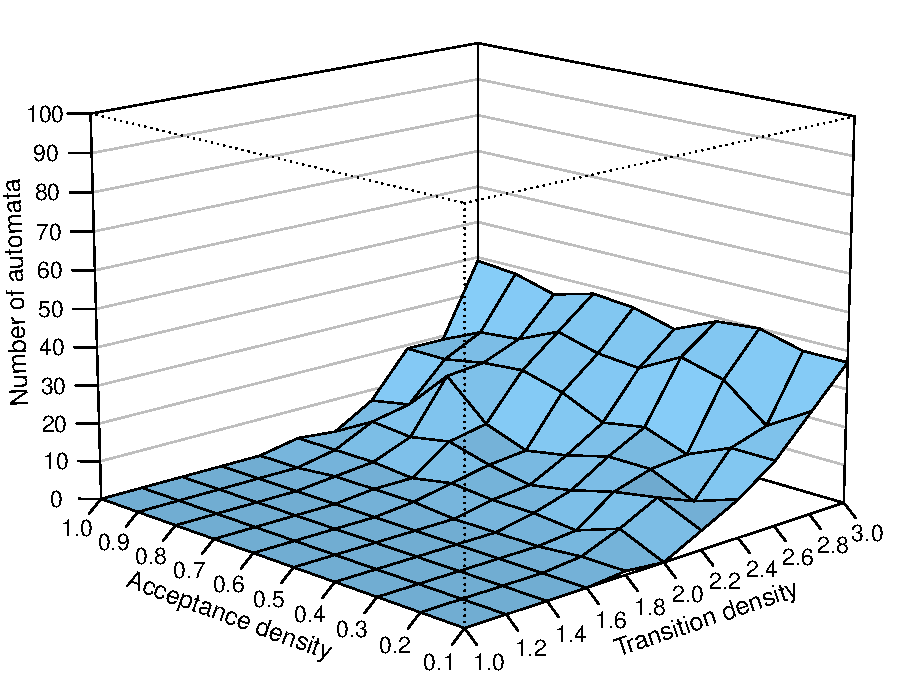
\includegraphics[width=\textwidth]{figures/r/testset/compl.persp.pdf}
    \end{subfigure}
  \caption{Number of \textit{complete} automata per class.}
  \end{subfigure}

 \begin{subfigure}{\textwidth}
    \begin{subtable}{0.47\textwidth}
    % latex table generated in R 3.1.2 by xtable 1.7-4 package
% Sun Aug 16 12:48:04 2015
\begin{tabular}{r|RRRRRRRRRR}
  & 0.1 & 0.2 & 0.3 & 0.4 & 0.5 & 0.6 & 0.7 & 0.8 & 0.9 & 1.0 \\ 
  \hline
1.0 & 4 & 5 & 5 & 7 & 8 & 4 & 6 & 10 & 4 & 3 \\ 
  1.2 & 1 & 3 & 5 & 8 & 8 & 12 & 10 & 13 & 4 & 14 \\ 
  1.4 & 2 & 17 & 13 & 17 & 20 & 24 & 22 & 21 & 27 & 26 \\ 
  1.6 & 16 & 28 & 30 & 37 & 49 & 42 & 42 & 49 & 45 & 45 \\ 
  1.8 & 31 & 40 & 55 & 59 & 64 & 67 & 76 & 70 & 63 & 78 \\ 
  2.0 & 60 & 64 & 85 & 75 & 83 & 83 & 79 & 90 & 87 & 83 \\ 
  2.2 & 67 & 87 & 86 & 88 & 89 & 91 & 89 & 89 & 89 & 86 \\ 
  2.4 & 88 & 89 & 86 & 92 & 95 & 95 & 94 & 97 & 96 & 97 \\ 
  2.6 & 86 & 93 & 92 & 97 & 97 & 97 & 98 & 96 & 98 & 96 \\ 
  2.8 & 94 & 97 & 95 & 94 & 97 & 99 & 98 & 97 & 97 & 100 \\ 
  3.0 & 99 & 99 & 99 & 97 & 99 & 98 & 100 & 100 & 100 & 99 \\ 
  \end{tabular}

    \end{subtable}
    \hfill
    \begin{subfigure}{0.52\textwidth}
    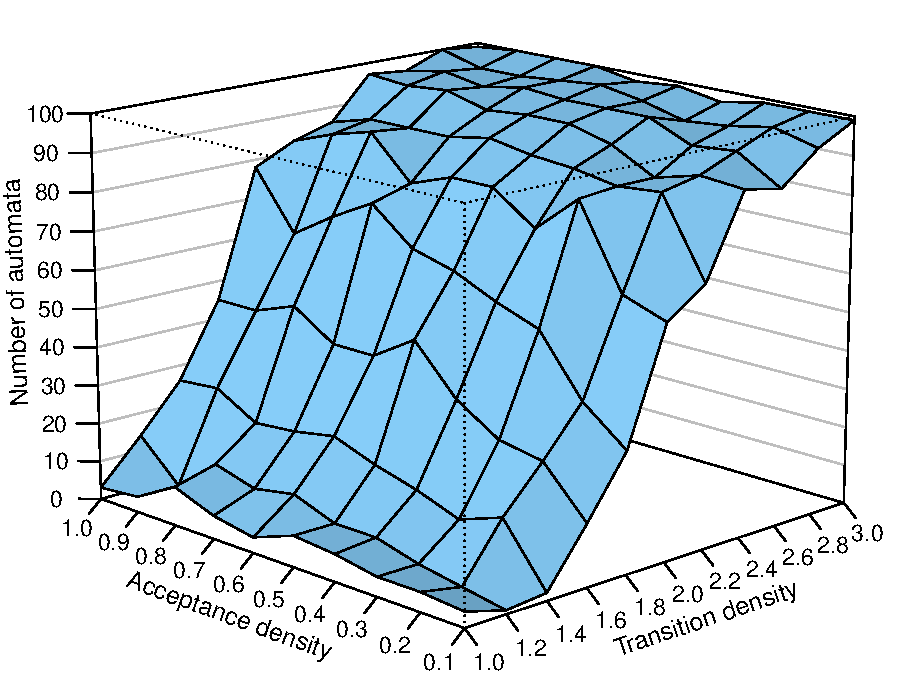
\includegraphics[width=\textwidth]{figures/r/testset/univ.persp.pdf}
    \end{subfigure}
  \caption{Number of \textit{universal} automata per class}
  \end{subfigure}

  \begin{subfigure}{\textwidth}
    \begin{subtable}{0.47\textwidth}
    % latex table generated in R 3.1.2 by xtable 1.7-4 package
% Sun Aug 16 12:48:05 2015
\begin{tabular}{r|RRRRRRRRRR}
  & 0.1 & 0.2 & 0.3 & 0.4 & 0.5 & 0.6 & 0.7 & 0.8 & 0.9 & 1.0 \\ 
  \hline
1.0 & 17 & 7 & 4 & 5 & 2 & 4 & 3 & 1 & 1 & 0 \\ 
  1.2 & 4 & 2 & 1 & 1 & 0 & 1 & 0 & 0 & 0 & 0 \\ 
  1.4 & 2 & 1 & 0 & 0 & 0 & 0 & 0 & 0 & 1 & 2 \\ 
  1.6 & 0 & 0 & 0 & 0 & 0 & 0 & 1 & 0 & 0 & 0 \\ 
  1.8 & 1 & 0 & 0 & 0 & 1 & 0 & 0 & 0 & 0 & 0 \\ 
  2.0 & 0 & 0 & 0 & 0 & 0 & 0 & 0 & 0 & 0 & 0 \\ 
  2.2 & 0 & 0 & 0 & 0 & 0 & 0 & 0 & 0 & 0 & 0 \\ 
  2.4 & 0 & 0 & 0 & 0 & 0 & 0 & 0 & 0 & 0 & 0 \\ 
  2.6 & 0 & 0 & 0 & 0 & 0 & 0 & 0 & 0 & 0 & 0 \\ 
  2.8 & 0 & 0 & 0 & 0 & 0 & 0 & 0 & 0 & 0 & 0 \\ 
  3.0 & 0 & 0 & 0 & 0 & 0 & 0 & 0 & 0 & 0 & 0 \\ 
  \end{tabular}

    \end{subtable}
    \hfill
    \begin{subfigure}{0.52\textwidth}
    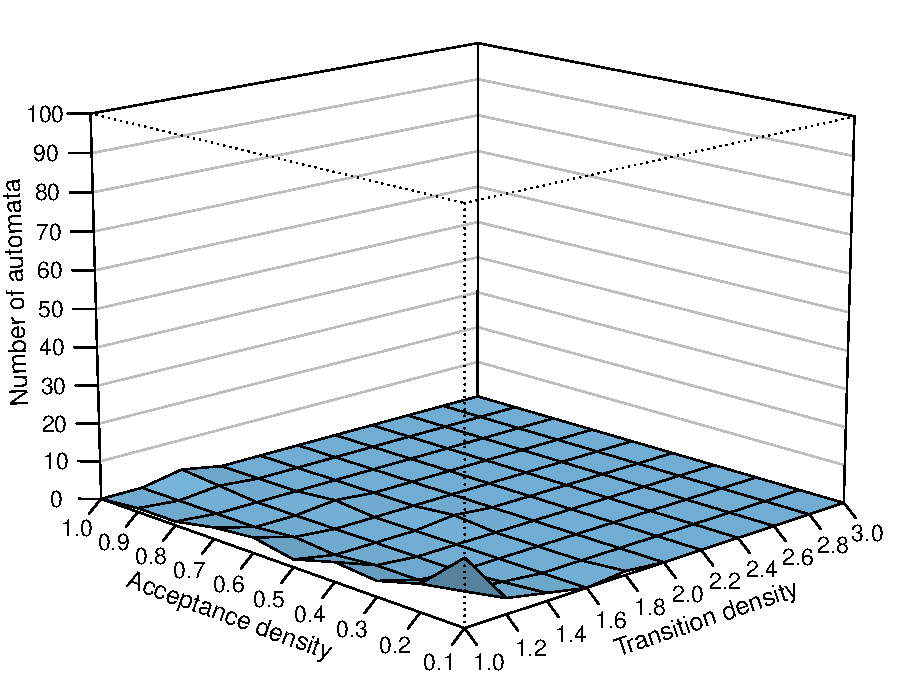
\includegraphics[width=\textwidth]{figures/r/testset/empt.persp.pdf}
    \end{subfigure}
  \caption{Number of \textit{empty} automata per class}
  \end{subfigure}
\caption{Number of complete, universal, and empty automata in each of the 110 transition density/acceptance density classes of the \goal{} test set. Note that each class contains 100 automata.}
\label{testset_analysis}
\end{figure}
\tablestyle  % Reset old table spacings

We tested all the automata in the \goal{} test set for completeness, universality, and emptiness. It is interesing to know about these special cases of automata because they may have an effect on the complementation results. The ideal complement of an empty or universal automaton has a size of one. Thus, by comparing this against the number of actually produced states, the number of ``superfluous'' states that the construction generated becomes apparent. Regarding completeness, the R2C optimisation applies only to complete automata, thus it is interesting to see on which automata this optimisation has in fact an effect.

\goal{} provides a command for testing emptiness. However, it does not provide commands for testing completeness and universality. Therefore, we implemented these commands on our own and bundled them as a separate \goal{} plugin. This plugin is called \textsf{ch.unifr.goal.util} and is also available as described in Appendix~\ref{app_plugin}.

With these \goal{} commands we tested and recorded for each of the 11,000 automata whether it is complete, unviversal, or empty. We then determined the number of complete, universal, and empty automata in the entire test set, as well as in each of the 110 transition density/acceptance density classes. The number of complete, universal, and empty automata in the entire test set of 11,000 automata are as follows:

\begin{itemize}
\item 990 complete automata (9\%)
\item 6,796 universal automata (61.8\%)
\item 63 empty automata (0.6\%)
\end{itemize}

The fact that only 9\% of the automata are complete means that the R2C optimisation of the Fribourg construction affects only 9\% of the test data. This is an interesting fact for the analysis of the effect the R2C optimisation has on the overall performance of the construction. A surprisingly high number of 61.8\% of the automata are universal. A reason for this might be the small alphabet consisting of only two symols of the automata. With a certain number of transitions in the automata, there seems to be a high probability that the automata are universal. Conversely, the number of empty automata is very low. This can be seen as the reverse of the same effect that causes the number of universal automata to be high.

In Figure~\ref{testset_analysis}, we show the number of complete, universal, an d empty automata for each of the 110 classes. By the way, in this figure we introduce two ways for representing per-class data that we will use throughout this thesis. On the left side of Figure~\ref{testset_analysis} the per-class data is represented as matrices. These matrices always have 11 rows and 10 columns, and the rows always represent the transition densities and the columns represent the acceptance densities. On the right side of Figure~\ref{testset_analysis}, the same data is visualised as so called perspective plots. The corner of the perspective plots that is closest to the viewer corresponds to the upper-left corner of the corresponding matrices. Thus, looking at a perspective plots is like looking at the corresponding matrix from beyond the upper-left corner. The advantage of matrices is that they show all the data values explicitly. The advantage of perspective plots is that they show the patterns in the data more intuitively. When we present the results of our study in Chapter~\ref{chap_results}, we mainly use perspective plots, however, we provide all the corresponding matrices in Appendix~\ref{app_matrices}.

Regarding the complete automata per class in Figure~\ref{testset_analysis}~(a), we can see that their number increases with the transition density. Up to a transition density of 1.6 there are no complete automata at all, and then it starts to increase up to a number between 34 and 40 for the transition density of 3.0. Since each class contains exactly 100 automata, these numbers can similarly be viewed as percentages. That the number of complete automata increases with the transition density is because a higher number of transitions per alphabet symbol in the automaton increases the probability that each state has at least one outgoing transition for each alphabet symbol. For example, with a transition density of 1.0 and 15 states, the automaton contains exactly 15 transitions for each alphabet symbol. It is still possible that this automaton is complete, but the probability is very low, because there must be a one-to-one mapping of transitions and states. On the other hand, with a transition density of 3.0, there would be 45 transitions per alphabet symbol, and the probability that each state gets one of them is much higher.

The number of universal automata per class in Figure~~\ref{testset_analysis}~(b) also increases with the transition density, although much stronger. While in the classes with a transition density of 1.0, there are between 3 and 10 universal automata, in the classes with a transition density of 3.0 there are between 97 and 100. As already mentioned, the small alphabet size of the \goal{} test set automata and a sufficiently high number of transitions results in a high probability that an automaton accepts every possible word, and thus is universal. In Figure~\ref{testset_analysis}~(b) we can also see that low acceptance densities result by trend in slightly fewer universal automata. This is because with fewer accepting states there is less chance that a given word is accepted. As we identified the small alphabet size as a possible reason for the high number of universal automata, it would be interesting to investigate the number of universal automata in automata with a bigger alphabet size. We let this as an idea for future work.

Conversely to the high number of universal automata, the number of empty automata is very low. The totally 63 empty automata are mainly concentrated in the upper-left corner of the matrix in Figure~\ref{testset_analysis}~(c). That is, the automata with a low transition density and a low acceptance density have the highest probability to no accept any word, and thus being empty. The reasons for this is roughly the opposite reasons for the distribution of the universal automata.


\subsection{Michel Test Set}
\label{4_michel_testset}
The Michel test set is very different from the \goal{} test set. It consists of only four automata, that however exhibit an exceptionally high state growth. Michel automata have been introduced in 1988 by Michel~\cite{michel1988} in order to prove a lower bound for the worst-case state complexity of Büchi complementation of $(n-2)!$~\cite{1996_thomas}. The Michel autoamate are characterise by the parameter $m$. They have an alphabet size of $m+1$, and $m+2$ states. Michel proved that the complements of these automata cannot have less than $m!$ states. Since the number of states of the input automata is $n = m + 2$, the minimum state growth of these automata is $(n-2)!$.

In practice, however, the state growth that is obseved for Michel automata is much higher. It is so high that for practical reasons we are restricted to include only the first four Michel automata with $m=\{1,\dots,4\}$ in our test set. For the Michel automata with $m \geq 5$, the required time and computing power for complementing them with our implementation would by far exceed our available resources. We present extrapolations toward larger Michel automata in Section~\ref{5_internal_michel}. Despite the small number of tested automata, we still obtain very interesting results, as we will see in Chapter~\ref{chap_results}.

The four Michel automata in our test set are shown in Figure~\ref{michel_automata}. We will call them Michel~1, Michel~2, Michel~3, and Michel~4, respectively. As mentioned, Michel automata have $m+2$ states and an alphabet size of $m+1$. Furthermore, they all have a single accepting state. Our Michel automata 1 to~4 have thus 3, 4, 5, and 6 states, and alphabet sizes of 2, 3, 4, and 5, respectively.

\renewcommand{\subwidth}{0.42}
\begin{figure}[htb!]
\centering
  \begin{subfigure}[t]{\subwidth\textwidth}
  \MichelOne
  \caption{Michel 1 ($m=1$)}
  \end{subfigure}
  \begin{subfigure}[t]{\subwidth\textwidth}
  \MichelTwo
  \caption{Michel 2 ($m=2$)}
  \end{subfigure}

  \begin{subfigure}[b]{\subwidth\textwidth}
  \MichelThree
  \caption{Michel 3 ($m=3$)}
  \end{subfigure}
  \begin{subfigure}[b]{\subwidth\textwidth}
  \MichelFour
  \caption{Michel 4 ($m=4$)}
  \end{subfigure}
\caption{The Michel automata with $m = \{1,\dots,4\}$, an alphabet size of $m+1$, and $m+2$ states.}
\label{michel_automata}
\end{figure}

It is interesing to use Michel automata to investigate the performance of Büchi complementation constructions, because they force the constructions to generate large number of states. By furthermore using several Michel automata with different sizes, it is possible to fit a state growth function on the resulting complement sizes. The state growth observed from the Michel automata is most likely not equal to the worst-case state growth (there are even worse automata), but it still provides a lower bound for the worst-case state growth. This can be interesting in case the worst-case state growth has not yet been precisely determined.  This function will certainly not be equal to the theoretical state growth function, but it still provides a lower bound for the worst-case state growth


\section{Experimental Setup}
\label{4_exp_setup}
In this section, we describe the experimental setup of our empirical performance investigation. This includes the specification of the concrete constructions (or versions of constructions) that are tested, constraints that are imposed on the runs, and the execution environment. As mentioned, the investigation is divided into the internal tests and external tests. In the internal tests we compare different versions of the Fribourg construction with each other. In the external tests, we compare one of the versions of the Fribourg construction with a set of different complementation constructions.

In Section~\ref{4_internal}, we present the tested verions for the internal tests. These versions differ for the \goal and the Michel test set, and we present them separately. In Section~\ref{4_external}, we present the tested constructions (including one of the versions of the Fribourg construction) for the external tests. In Section~\ref{4_exec_env}, we describe the computing environment in which the experiments were executed. Finally, in Section~\ref{4_limits}, we present the time and memory limits that were imposed on the individual executions. 

\subsection{Internal Tests}
\label{4_internal}
The versions of the Fribourg construction used for the internal tests consist of combinations of the three optimisations R2C, M1, and M2, and of the additional options C and R (see list of options for the Fribourg construction in Table~\ref{goal_options}). The sets of versions are different for the \goal{} and the Michel test set.

\subsubsection{GOAL Test Set}
For the internal tests on the GOAL test set, we use the following eight versions of the Fribourg construction:
\begin{enumerate}
\item Fribourg
\item Fribourg+R2C
\item Fribourg+R2C+C
\item Fribourg+M1
\item Fribourg+M1+R2C
\item Fribourg+M1+R2C+C
\item Fribourg+M1+M2
\item Fribourg+R
\end{enumerate}

The first version, Fribourg, is the plain Fribourg construction without any optimisations or options. The next two versions, Fribourg+R2C and Fribourg+R2C+C, aim at investigating the R2C optimisation. In Fribourg+R2C, the R2C optimisation is applied only to complete input automata. As we have seen in Section~\ref{4_goal_testset} these are just 9\% of the automata. Fribourg+R2C+C, on the other hand, makes the incomplete input automata complete so that the R2C optimisation is applied to all automata. The fact that we want to find out is whether it is worth to increase the size of an automaton by one (for adding the sink state) for the sake of being able to apply the R2C optimisation.

A very similar question has been investigated in previous work on the Fribourg construction by Göttel~\cite{2013_bsc_goettel}. In terms of our above listing, he compares the performance of Fribourg with Fribourg+R2C+C. As the test data, he also uses the \goal{} test set. His results are that the overall mean complement size resulting from Fribourg+R2C+C is higher than for Fribourg. However, by looking closely at Göttel's results we suppose that the median complement size (which is not reported in~\cite{2013_bsc_goettel}) might be lower for Fribourg+R2C+C than for Fribourg. This would be an interesting relation, and therefore, we decided to re-investigate this question. 

Fribourg+M1 and Fribourg+M1+M2 aim at investigating the M1 and M2 optimisations. As M2 can only be applied together with M1, there are only these two possible combinations. As we will see in Chapter~\ref{chap_results}, Fribourg+M1 shows a better performance on the \goal{} test set than Fribourg+M1+M2. Therefore, we do not further investigate any versions based on Fribourg+M1+M2, however, we further investigate versions based on Fribourg+M1. This is why the next two versions are Fribourg+M1+R2C and Fribourg+M1+R2C+C. With these versions, we investigate the effect of the R2C optimisation in combination with the M1 optimisation. The last version, Fribourg+R, corresponds to the first version, Fribourg, but with the difference that in Fribourg+R all unreachable and dead states are removed from the output automaton. This allows to determine the number of unreachable an dead states that have been produced by Fribourg.

The versions Fribourg+M1+R2C and Fribourg+M1+R2C+C enhance the ``better'' of Fribourg+M1 and Fribourg+M1+M2 with R2C and R2C+C, respectively. As we will see in Chapter~\ref{chap_results}, the better one of these two versions terms of median complement sizes is Fribourg+M1. That is, the application of M2 results in a decline, rather than a gain, in performance compared to the application of M1 alone. It is imporant to highlight that such results are specific to the used test data, and not universally valid. With different test data Fribourg+M1+M2 might be better than Fribourg+M1. As we will see in the next section, this is for example the case for our Michel test.

The last version, Fribourg+R, corresponds to the application of the plain Fribourg construction without any optimsations or options, but with the difference that at the end of the construction all unreachable and dead states are removed from the complement automaton. Comparing the results of Fribourg+R with the results of Fribourg reveals how many unreachable and dead states the Fribourg construction produces. This idea is inspired by the study by Tsai et al.~\cite{2011_tsai} in which the number of unreachable and dead states is one of the main performance metrics for the tested constructions..

\subsubsection{Michel Test Set}
For the internal tests on the Michel test set, we use the following six versions of the Fribourg construction:
\begin{enumerate}
\item Fribourg
\item Fribourg+R2C
\item Fribourg+M1
\item Fribourg+M1+M2
\item Fribourg+M1+M2+R2C
\item Fribourg+R
\end{enumerate}

The rationale behind the selection of these versions is basically the same as for the GOAL test set. However, there are the following differences. First, the Michel automata are complete, thus there is no need to include the C option. Second, for the Michel test set, Fribourg+M1+M2 is more performant than Fribourg+M1. This is why Fribourg+M1+M2+R2C is based on Fribourg+M1+M2 rather than Fribourg+M1.


\subsection{External Tests}
In the external tests, we compare the results of the best version of the Fribourg construction on each test set, with the results of a set of other complementation constructions that are implemented in \goal. As already mentioned, the best versions of the Fribourg constructions on the two test sets turn out to be the following:

\begin{itemize}
\item Fribourg+M1+R2C \tabto{4.2cm} for the \goal{} test set
\item Fribourg+M1+M2+R2C \tabto{4.2cm} for the Michel test set
\end{itemize}

Regarding which other complementation constructions to use, we principially could use all the constructions listed in Table~\ref{goal_constructions}. However, in preliminary tests we observed that most of these constructions are not performant enough to be reasonably used with the \goal{} test set. Using them would require to allocate very high time and memory resources. Tsai et al.~\cite{2011_tsai} made a similar experience with these constructions in \goal when they observed that Ramsey could not complete any of the 11,000 complementation tasks in the \goal{} test set within the time limit of 10 minutes and a memory limit of 1 GB. 

 % According to our tests, this excludes all but  Piterman, Slice, Rank, and Safra from being reasonably used. A similar experience has been made by Tsai~et~al. in their own empirical study~\cite{2011_tsai}. They observed that the Ramsey construction could not complement \textit{any} of the 11,000 automata in the \goal{} test set within the time limit of 10 minutes and memory limit of 1 GB.

There are three constructions that are performant enough to be used with the \goal{} test set for our purposes, namely Piterman, Slice, and Rank. For this reason, we only include these three constructions in the external tests\footnote{Actually, Safra would also be performant enough, but since we can use Piterman, which is an improvement of Safra, we chose to not include Safra.}. Interestingly, these constructions represent three of the four main complementation approaches, namely the determinisation-based (Piterman), the rank-based (Rank), and the slice-based (Slice) approach. In detail we use the following constructions for the external tests:

\begin{itemize}
\item Piterman+EQ+RO
\item Slice+P+RO+MADJ+EG
\item Rank+TR+RO
\end{itemize}

Note that regarding the options, we include those options for each construction which are set as default in their implementation, except the MACC (maximise accepting set of input automaton) and R (remove unreachable and dead states of output automaton) options, because they are not part of the constructions, but rather pre-processing and post-processing steps\footnote{For Piterman, we also exclude the SIM option, which is set by default. This is because it simplifies the intermediate complement parity automaton, which can be seen as a post-processing step.}. Some of the used options are described by Tsai et al. in~\cite{2011_tsai}, in which case we indicate it below.

Piterman+EQ+RO is the determinisation-based construction by Piterman~\cite{2006_piterman,2007_piterman} with the EQ and RO options of its implementation in \goal. These options are described in \goal{} as follows:
\begin{itemize}
\item EQ: merge equivalent states during the conversion of the complement parity automaton to the complement Büchi automaton (described in~\cite{2011_tsai})
\item RO: reduce transitions in the conversion from the complement parity automaton to the complement Büchi automaton
\end{itemize}

Slice+P+RO+MADJ+EG is the construction by Vardi and Wilke~\cite{vardi2007automata} with the RO, MADJ, and EG options (note that the P option causes the usage the construction by Vardi and Wilke~\cite{vardi2007automata}, as opposed to the construction by Kähler and Wilke~\cite{2008_kaehler}, which is used without the P option). The options have the following meaning:
\begin{itemize}
\item RO: reduce the out-degree of states
\item MADJ: merge adjacent 0-components or $*$-components (described in~\cite{2011_tsai})
\item EG: use enhanced guessing (described in~\cite{2011_tsai})
\end{itemize}

Rank+TR+RO is the rank-based construction by Schewe~\cite{schewe2009buchi} with the TR and RO options. The meaning of these options is as follows:
\begin{itemize}
\item TR: use tight rankings
\item RO: reduce the out-degree of states
\end{itemize}

Note that in Chapter~\ref{chap_results}, we refer to these three construction as Piterman, Slice, and Rank, for short. However, what we actually mean are the three precise versions as described above.


% Considering these restrictions, we decided to include only Piterman, Slice, and Rank in our external tests. These constructions furthermore represent three of the four main complementation approaches, namely the determinisation-based, rank-based, and slice-based approach. The fourth approach would be Ramsey-based, however, as mentioned the implementation of the Ramsey-based construction by Sistla et al.~\cite{1985_sistla} in \goal{} is not efficient enough for our study. It would have been possible to also include Safra. However, as we include Piterman, which is in fact an improvement of Safra (see Section~\ref{2_determinisation-based}, we decided that it is not necessary to additionally include Safra. 

% For Slice, we actually use the construction that is indicated as Slice+P in Table~\ref{goal_constructions}. Slice+P is the construction by Vardi and Wilke~\cite{vardi2007automata}, whereas Slice is the consruction by Kähler and Wilke~\cite{2008_kaehler}. Since the construction by Vardi and Wilke is more efficient than the construction by Kähler and Wilke (see Section~\ref{2_slice-based}), we decided to use Vardi and Wilke's construction, that is Slice+P. Note that in the following, we will nevertheless refer to this construction as Slice, however, we mean by this at any point Vardi and Wilke's construction~\cite{vardi2007automata}.

% Piterman, Rank, and Slice also have a set of selectable optimisations in \goal{} (some of these optimisations have been proposed by Tsai et al.~\cite{2011_tsai}). We decided to include the set of optimisations for each of the three constructions that is activated by default in \goal, except the MACC and R optimisations. The reason to exclude MACC and R is that they are not part of the actual construction, but rather just modify the input automaton before the construction starts, or the output automaton after the construction ends, respectively. By otherwise using the default optimisations, we are likely to use the most optimal versions of these constructions. This makes the comparison with the Fribourg construction fair, because for the Fribourg construction we also choose the most optimal version for the external tests.

% Note that for Piterman, we also exclude the SIM optimisation, even though it is set by default in \goal. This is because the SIM optimisation of Piterman simplifies the complement DPW of the construction. This can be seen as a similar optimisation as the R option, and thus, we do not want to include it in our tests.

% Using the optimisations for Piterman, Slice, and Rank according to these rules, we obtain the precise versions Piterman+EQ+RO, Slice+P+RO+MADJ+EG, and Rank+TR+RO. Regarding the Fribourg construction, we use the best versions for each of the two test sets. As we will see in Chapter~\ref{chap_results}, these are Fribourg+M1+R2C for the \goal{} test set, and Fribourg+M1+M2+R2C for the Michel test set.

% Consequently, for the \goal{} test set, the tested constructions are:

% \begin{enumerate}
% \item Piterman+EQ+RO
% \item Slice+P+RO+MADJ+EG
% \item Rank+TR+RO
% \item Fribourg+M1+R2C
% \end{enumerate}

% For the Michel test set, on the other hand, the tested constructions are:

% \begin{enumerate}
% \item Piterman+EQ+RO
% \item Slice+P+RO+MADJ+EG
% \item Rank+TR+RO
% \item Fribourg+M1+M2+R2C
% \end{enumerate}


% Justification to use only Piterman, Slice, and Rank
% UBELIX/jobs/2014-10-09:
% Complemented the first 10 of the size-15 test set with all constructions, and only Piterman, Slice, Rank, and Safra completed all of them.
% See Tsai (2011) page 5: they compared Ramsey, Piterman, Rank, and Slice. But Ramsey couldn't complement any of the 11,000 automata of size 15 within the time nd memory limits
% Ramsey, Piterman, Rank, and Slice are representative for the four main complementatio approaches, Ramsey-based, determinization-based, rank-based, and slice-based.

\subsection{Time and Memory Limits}
\label{4_limits}
Similarly to Tsai et al.~\cite{2011_tsai}, we set a time and  a memory limit for each complementation task of the \goal{} test set. The time limit is 600 seconds (10 minutes) CPU time, and the memory limit is 1 GB for the Java heap memory. These limits roughly conincide with the limits in~\cite{2011_tsai}, which are also 10 minutes and 1 GB, however, it is not specified whether the 10 minutes are CPU time or real time, and whether 1 GB applies to the process' entire memory, or to a portion of it, like the Java heap. Complementation tasks that exceed the time or memory limit are aborted, and consequently do not deliver any results.

Note that these limits apply only to the \goal{} test set. For the Michel test set, we do not set any limits, because in this case there are only four automata, and we want each of them to be completed.

% We imposed a time and memory limit on every complementation task of the \goal{} test set. For the Michel test set, we did not set any limits, because it consists of a much smaller number of tasks. These limits are based on the limits that have been used by Tsai et al.~\cite{2011_tsai}. Our time limit is 600 seconds CPU time, and our memory limit corresponds to 1 GB Java heap. If a complementation taks is not finished after 600 seconds CPU time, or requires more than 1 GB heap memory, then the tasks aborted.

The reasons for these limits are restricted computing and time resources. Clearly, the ideal case would be to let every complementation task run to completion, no matter how long it takes and how much memory it uses. However, because of the high complementation complexity that Büchi automata may have, some few extreme cases may cause our available resources to be exceeded\footnote{As we will see in Chapter~\ref{chap_results}, the distribution of the complexity of the tested Büchi automata is extremely right-skewed, that is, most are easy, and very few are hard.}. The study is for example ultimately limited by the physically available memory on the nodes, and the maximum running time of a job permitted by the cluster mangement software. Wit these limits we can thus cut off such extreme cases and keep the required resources for the study in affordable bounds.

We implemented the time limit by the means of the \textsf{ulimit} Bash builtin, which allows to set a maximum running times for processes. Processes that reach this time limit are aborted by the operating system.

The memory limit, as mentioned, defines the maximum size of the Java heap. The heap is the main memory area of the Java process. It is where all the objects that are created by the Java program are stored. Concretely, this means that the states of the complements that are generated by the tested constructions are stored on the heap. It is possible to set the maximum Java heap size with the \textsf{Xmx} option to the Java Virtual Machine\footnote{Example usage: \textsf{java -Xmx1G}}. We also set the initial size of the Java heap to 1 GB by the means of the \textsf{Xms} option, so that the heap does not need to be enlarged what could distort the measured execution times.

The presence of time and memory limits, and thus aborted complementation tasks, require the use of so-called \textit{effective samples}. The concept of effective samples is also used by Tsai et al.~. These limits are based on the limits that have been used by Tsai et al.~\cite{2011_tsai}. The effective samples are those automata which have been successfully completed by \textit{all} constructions that are compared to each other. Imagine, for example, two constructions $C_1$ and $C_2$ that are used to complement a test set of 1,000 automata. $C_1$ successfully complements all the automata, whereas $C_2$ gets aborted for 100 of these automata. If we would statistically evaluate and compare the 1,000 results of $C_1$ and the 990 results of $C_2$, then $C_2$ would be advantaged, because the results of the 100 apparently hardest automata are not taken into account, whereas they are included in the evaluatio of $C_1$. This is why in this case only the 990 effective samples that have been successfully completed by both constructions must be evaluated. In Chapter~\ref{chap_results}, we will therefore only evaluate the effective samples of the compared constructions.


\subsection{Execution Environment}
\label{4_exec_env}
Due to the computational intensity, we executed all the complementation tasks, that we outlined in the last section, on a HPC computer cluster. In particular, we used the computer cluster named UBELIX of the University of Bern\footnote{\url{http://ubelix.unibe.ch}}. Note that we also executed the correcntess tests for the implementation of the Fribourg construction (see Section~\ref{4_verification}) and the analysis of the \goal{} test set (see Section~\ref{4_goal_test_set}) on UBELIX.

Generally, a computer cluster consists of interlinked \textit{nodes} (computers) on which the \textit{jobs} (computation tasks) of the users of the clusters are run. Typically, cluster users submit their jobs to a cluster management software, which automatically dispatches these jobs to suitable and available nodes. In the case of UBELIX, this cluster management software is Oracle Grid Engine (formerly known as Sun Grid Engine) version 6.2\footnote{\url{http://www.oracle.com/us/products/tools/oracle-grid-engine-075549.html}}.

We ensured that all our tasks are executed on similar nodes. These nodes have the following specifications:
\begin{itemize}
\item Processor: Intel Xeon E5-2665 2.40GHz
\item Architecture: 64 bit
\item CPUs (cores): 16
\item Memory (RAM): 64 GB or 256 GB
\item Operating System: Red Hat Enterprise Linux 6.6
\item Java platform: OpenJDK Java 6u34
\item Shell: GNU Bash 4.1.2
\end{itemize}

Note that the memory of the nodes is either 64 GB or 256 GB. The tasks on the \goal{} test set were run on nodes with 64 GB RAM, the tasks on the Michel test set on special high-memory nodes with 256 GB RAM. Apart from that, the specifications of these nodes are identical. The use of the high-memory nodes for the Michel test set was required, because the maximally allocatable memory per CPU of the nodes with 64 GB memory is 4 GB, and this was not enough to complement the Michel automata. With the high-memory nodes, on the other hand, a total of 16 GB can be allocated per CPU which was sufficient to complement all the Michel automata.

Regarding multicore usage, the behaviour of our tasks depends on \goal, and thus ultimately on Java. \goal{} is multi-threaded and thus our taks may use  multiple CPUs. Theoretically, they can use up to the total number of 16 CPUs of a node. However, we observed that our tasks typically used between two and four CPUs\footnote{We can just indirectly guess this number by comparing the measured CPU times and real times of concrete tasks.}.

We also measured the execution time of each complementation task as CPU time and real time (also known as wallclock time). The CPU time is the time a process is actually executed by the CPU. The real time is the time that passes from the start of a process until its termination, and thus includes the time the process is not executed by the CPU (idle time). These measurements were done with Bash's \textsf{time} reserved word. If a process runs on multiple CPUs, the CPU time is counted on each CPU separately and finally summed up. This means that for multicore execution (as in our case), the CPU time may be higher than the real time. For single-core execution, on the other hand, this is not possible, and the CPU time may only be equal to or lower than the real time. In the analysis of our results in Chapter~\ref{chap_results}, we sometimes present statistics of the execution times. These times are always \textit{CPU times}.

The complementation tasks are executed sequentially via the command line interface of \goal. For each complementation task the \goal{} application is started separately, which includes the loading of the Java Virtual Machine (JVM). The JVM startup time is thus included in our measured execution times, and acts like a constant. According to our observations, the JVM startup time is approximately two CPU time seconds.

A computer cluster is a multi-user environment and a node can be used by multiple users at the same time. Thus, the total load of a node may vary, depending on number and intensity of other users' jobs. Our tasks were also subject to varying node loads. We do not know whether this has an influence on our experiments, in particular, on the measurement of the execution times, and on the imposed time limit (see next section). The load of a node has however  no influence on the complements that are produced by the complementation constructions, which is after all our main interest. Hence, we leave the topic of the influcence of node load on execution time for future work.\footnote{The idea of cluster usage is that each job has a requested number of CPUs exclusively for itself, in which case the used CPUs would not be affected of varying loads. However, jobs are not prevented from using more than the requested number of CPUs on the same node, what means that there is no guarantee that the used CPUs are not also used by other jobs, what may put them under varying load.}

% \begin{itemize}
% \item mpi.q
%   \begin{itemize}
%   \item hnode 01--42
%   \item Intel Xeon E5-2665 2.40GHz
%   \item 16 CPU cores (slots)
%   \item 64 GB RAM
%   \item $\rightarrow$ 4 GB RAM per core (slot)
%   \item h\_cpu limit: 72:00:00
%   \item h\_rt limit: 73:00:00
%   \end{itemize}
% \item highmem.q
%   \begin{itemize}
%   \item jnode 01--21
%   \item Intel Xeon E5-2665 2.40GHz
%   \item 16 CPU cores (slots)
%   \item 256 GB RAM
%   \item $\rightarrow$ 16 GB RAM per core (slot)
%   \end{itemize}
% \end{itemize}
% The tests are successful with the following resources:
% \begin{tabular}{|p{1.5cm}|l|r|r|r|r|r|p{3.5cm}|}
% \hline
% Test & Queue & Slots & \parbox[t]{1.75cm}{Job\\memory\\limit} & \parbox[t]{1.75cm}{Job CPU\\time limit} & \parbox[t]{1.75cm}{CPU time\\limit per\\automaton\\} & \parbox[t]{1.75cm}{Memory\\limit per\\automaton\\} & Notes \\
% \hline
% 1 and 2 & mpi.q & 4 & 4 GB & 72:00:00 & 600 sec. & 1 GB & rank -tr -ro has to be run on 10 partitions of the test set \\
% \hline
% 3 and 4 & highmem.q & 4 & 16 GB & 72:00:00 & None & 14 GB & piterman -eq -sim -ro out of memory on Michel N4 \\
% \hline
% 4 & mpi.q & 4 & 4 GB & 72:00:00 & None & 1 GB & \\
% \hline
% 5 & mpi.q & 4 & 4 GB & 72:00:00 & None & 2 GB & universal -m piterman -eq -ro \\
% \hline
% \end{tabular}

This concludes the present chapter that described the setup of our empirical performance investigation of the Fribourg construction. We explained how we implemented the Fribourg construction as a part of the \goal tool. Then, we presented our test data, consisting of the \goal{} test set and the Michel test set. Finally, we presented our experimental setup, specifying exactly which constructions wer are testing, under which constraints. In the next chapter, we present the results of this investigation.

